% !TEX root = ../main.tex
\ulfgchapter{2}{Radar Background and State of the Art}{chp:background}

\section{Introduction}

This chapter provides the background the rest of the report depends on, and reviews the published
work the results will later be compared against.

It has three parts. The first explains how an FMCW radar produces a range--Doppler map, because
that map is the input to every detector in this work. The second describes CFAR detection: the
principle, the main variants, and the failure modes that were documented decades ago and that
motivate learned alternatives. The third reviews learned detection on RD maps and argues that the
published literature separates into families whose results are not directly comparable. That
argument is used throughout the report, and it is the reason Chapter~\ref{chp:realdata} compares
against only a subset of the papers reviewed here.

Two results in this chapter are used directly later. The documented CFAR failure modes
(Section~\ref{sec:cfar_failures}) determine which conditions the synthetic benchmark of
Chapter~\ref{chp:synthetic} must contain. The equivalence between CA-CFAR and a convolution
(Section~\ref{sec:cfar_as_conv}) is what justifies treating a small convolutional network and CFAR
as two instances of the same operator, rather than as two unrelated systems placed side by side.

\section{FMCW radar principles}

\subsection{Chirp generation and the beat frequency}

An FMCW radar transmits a signal whose frequency increases linearly with time. One such sweep is
called a \emph{chirp}. The treatment here follows the standard
accounts~\cite{skolnik2001radar,richards2014radar}. Writing $B$ for the swept bandwidth and $T_c$ for the chirp duration, the
instantaneous frequency rises at a constant rate, the \emph{slope}
\begin{equation}
S = \frac{B}{T_c}.
\end{equation}

A target at range $R$ reflects the chirp back after a round-trip delay
\begin{equation}
\tau = \frac{2R}{c},
\end{equation}
where $c$ is the speed of light. The echo is therefore a copy of the transmitted chirp, shifted in
time. Because the frequency is ramping, a shift in time becomes a difference in frequency. Mixing
the echo with the transmitted signal and low-pass filtering the result --- an operation called
\emph{dechirping} --- produces a tone at the \emph{beat frequency}
\begin{equation}
f_b = S\,\tau = \frac{2BR}{c\,T_c}.
\label{eq:beat}
\end{equation}

Equation~\eqref{eq:beat} is the reason FMCW radar is inexpensive. Range has been converted into a
frequency of a few megahertz, so the receiver never has to sample at the radio frequency; it only
has to sample the beat tone. Figure~\ref{fig:chirp} shows the geometry for the radar used in this
work.

\begin{figure}[h!]
\centering
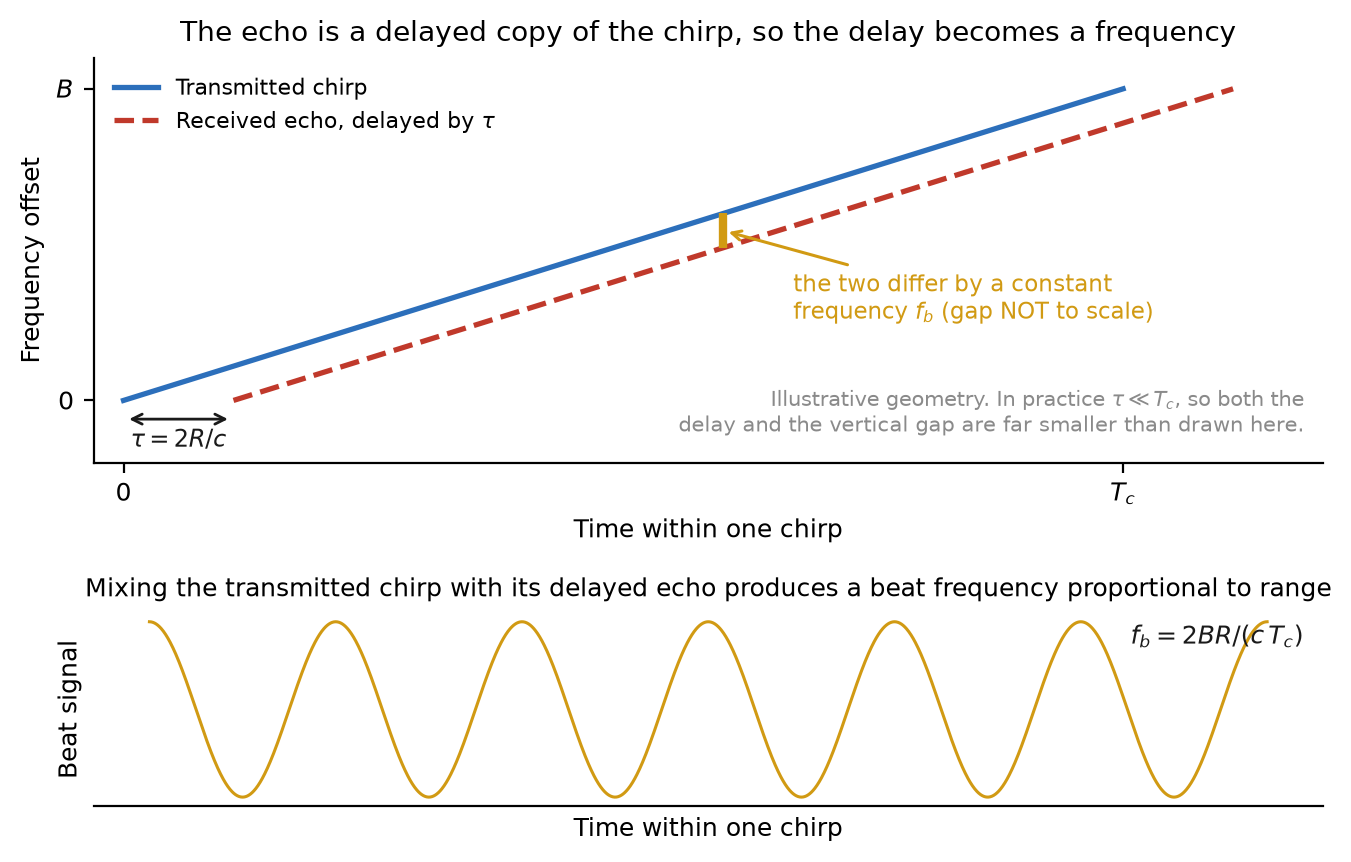
\includegraphics[width=0.92\textwidth]{figures/Chapter2/ch2_fig1_fmcw_chirp.png}
\caption[FMCW chirp geometry and the beat frequency]{Top: the received echo is a delayed copy of
the transmitted chirp, so mixing the two produces a beat frequency proportional to range. Axes are
normalised, in units of the swept bandwidth $B$ and the chirp duration $T_c$. The geometry is
illustrative: in practice $\tau \ll T_c$, so both the delay and the vertical gap labelled $f_b$ are
far smaller than drawn. Bottom: the resulting beat tone. The sensor parameters used in this work
are given in Chapter~\ref{chp:simulator}.}
\label{fig:chirp}
\end{figure}

\subsection{Range estimation}

Sampling the beat signal $N$ times within one chirp and applying a discrete Fourier transform
converts the tone into a peak at a known frequency bin. By equation~\eqref{eq:beat}, that bin
corresponds to a range. This first transform is called the \emph{range FFT}, and it is taken along
what is known as \emph{fast time}, meaning the samples within a single chirp.

As a nominal resolution criterion, two targets require approximately one range-resolution cell of
separation before they appear as separate peaks. This gives
\begin{equation}
\Delta R = \frac{c}{2B}.
\label{eq:range_res}
\end{equation}
The nominal FMCW range resolution is therefore determined primarily by the swept bandwidth, under
the standard assumptions of a linear sweep, an unwindowed transform and sufficient
signal-to-noise ratio. In particular it does not improve with a longer chirp, with higher
transmitted power, or at shorter target range. Window functions applied before the transform, which
suppress sidelobes, broaden the main lobe and so widen the achieved resolution beyond this nominal
value.

\subsection{Doppler estimation and the range--Doppler map}

A single chirp gives range but not velocity. Velocity is obtained by transmitting $M$ chirps in
quick succession and observing how the \emph{phase} of a target's beat tone changes from one chirp
to the next. A target moving radially changes its range slightly between chirps, and although that
change is far too small to move the target into a different range bin, it is a substantial fraction
of a wavelength and therefore produces a measurable phase rotation.

Taking a second Fourier transform across the $M$ chirps, at each range bin, converts that phase
rotation into a frequency: the Doppler shift. This transform is taken along \emph{slow time},
meaning across chirps. The relevant time step here is the \emph{chirp repetition interval} $T_r$,
the spacing between the starts of consecutive chirps, which in general is the chirp duration plus
any idle time between chirps. \textbf{The radar modelled in this work transmits chirps
back to back with no idle time, so $T_r = T_c$ throughout}; the two symbols are used
interchangeably from here on, and the simulator samples slow time at exactly this spacing. The
velocity resolution then follows the same reasoning as equation~\eqref{eq:range_res}:
\begin{equation}
\Delta v = \frac{\lambda}{2 M T_r},
\qquad
v_{\max} = \pm\frac{\lambda}{4 T_r},
\qquad T_r = T_c \text{ here},
\end{equation}
where $\lambda = c/f_c$ is the wavelength at carrier frequency $f_c$. Longer observation, meaning
more chirps, gives finer velocity resolution; a shorter repetition interval extends the unambiguous
velocity range.

The output of the two transforms is a two-dimensional array indexed by range bin and Doppler bin:
the \emph{range--Doppler map}. Each target appears as a localised concentration of energy at its
range and radial velocity. Figure~\ref{fig:chain} summarises the chain.

\begin{figure}[h!]
\centering
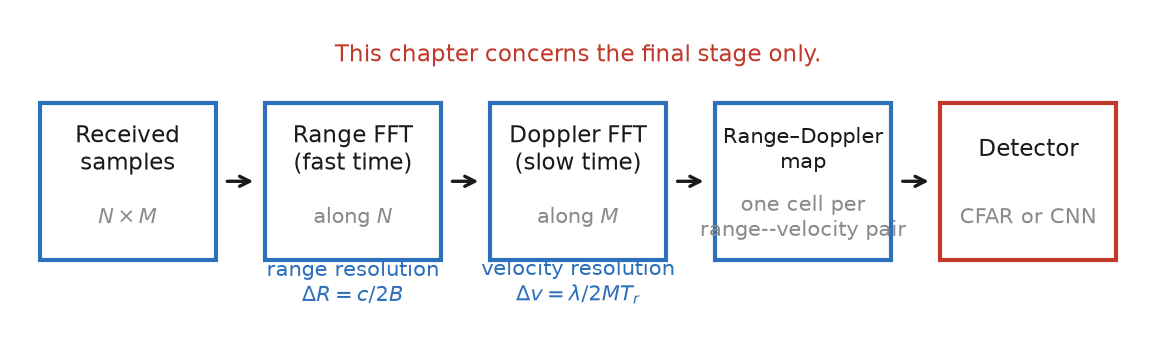
\includegraphics[width=\textwidth]{figures/Chapter2/ch2_fig2_processing_chain.png}
\caption[FMCW processing chain]{From received samples to the range--Doppler map. The detector,
which is the subject of this report, operates on the final stage only. The sensor parameters that
fix the two resolutions are specified in Chapter~\ref{chp:simulator}.}
\label{fig:chain}
\end{figure}

The RD map is an image, but it is not a photograph, and two of its properties matter for detection.
First, the background is not smooth: with a single look, the noise in each cell follows an
exponential power distribution, so neighbouring cells differ by many decibels purely by chance.
Second, a target is not a single bright pixel but a response spread over a few cells, set by the
window functions and the transform lengths rather than by the physical size of the object.
Figure~\ref{fig:rdmap} shows both effects on one frame of the benchmark used in this work.

\begin{figure}[h!]
\centering
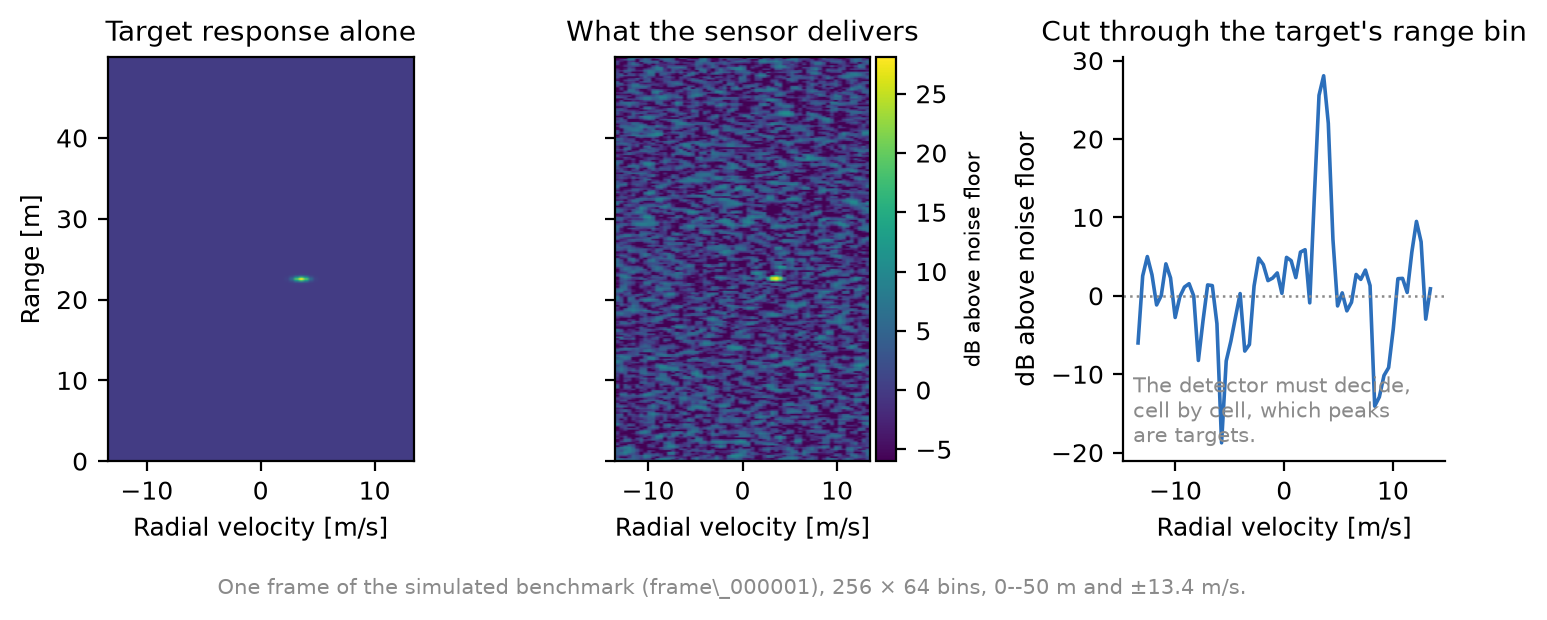
\includegraphics[width=\textwidth]{figures/Chapter2/ch2_fig3_rd_map_example.png}
\caption[A range--Doppler map and the detection problem]{Left: the target response on its own.
Centre: the same frame as the sensor delivers it. Right: a cut through the target's range bin. The
detector assigns scores or decisions to RD cells, after which local peaks are extracted as target
candidates; Chapter~\ref{chp:detectors} specifies that extraction step and makes it identical for
both detectors.}
\label{fig:rdmap}
\end{figure}

\section{Detection in the range--Doppler plane}

\subsection{The detection problem}

Detection is a binary hypothesis test applied to every cell of the RD map. Throughout this report
$x$ denotes the \emph{measured power} in an RD cell, that is the squared magnitude of the complex
range--Doppler sample, $x = |X|^2$. This is the output of a square-law detector, and it is a power
quantity rather than an amplitude; every threshold expression below is written in those units. For
a cell with measured power $x$, the two hypotheses are
\begin{align}
H_0 &: \text{background only (noise, clutter, interference)}, \\
H_1 &: \text{background plus a target return}.
\end{align}

Radar detectors are conventionally designed to the Neyman--Pearson criterion: fix the probability
of false alarm $\Pfa$ at an acceptable value, and maximise the probability of detection $\Pd$
subject to that constraint. This is the reason $\Pd$ at a fixed $\Pfa$ is the standard metric in
the field, and it is the metric this report uses.

Fixing $\Pfa$ is straightforward if the background power is known. Under the standard single-look
model the background power $x$ is exponentially distributed with mean $\sigma^2$, so
$\Pr(x > T \mid H_0) = \exp(-T/\sigma^2)$ and the threshold that achieves a chosen $\Pfa$ is
$T = -\sigma^2 \ln \Pfa$, again in units of power. The
difficulty is that $\sigma^2$ is not known. It varies with temperature, with the terrain being
illuminated, with weather, and with interference from other radars. A fixed threshold set for one
condition produces either a flood of false alarms or no detections at all in another.

\subsection{The constant false alarm rate principle}

CFAR detection solves this by estimating the background from the data itself. For each cell under
test, a window of surrounding cells is used to form an estimate $Z$ of the local background level,
and the threshold is set proportional to it:
\begin{equation}
T = \alpha Z,
\qquad
\text{decide } H_1 \text{ if } x > T.
\label{eq:cfar}
\end{equation}

The multiplier $\alpha$ is chosen so that the false-alarm rate takes the desired value. Because the
threshold scales with the estimated background, a uniform change in received power scales $x$ and
$Z$ together and leaves the decision unchanged. This is the constant false alarm rate property, and
it is what allows a single detector to operate across widely varying conditions.

It is worth being precise about what that property guarantees. The rate is held constant
\emph{under the assumed background model}: the reference cells are taken to be independent,
identically distributed and free of target energy, and to share the statistics of the cell under
test. When those assumptions hold, the achieved false-alarm rate is close to the design value
regardless of the absolute power level. When they do not hold --- at a clutter edge, where the
reference cells no longer share the statistics of the cell under test, or under target masking,
where they are not target-free --- the achieved rate can depart from the design value in either
direction. Section~\ref{sec:cfar_failures} describes both cases, and this departure is measured
rather than assumed in Chapter~\ref{chp:detectors}, which is why operating points in this report
are matched at the \emph{measured} rather than the design rate.

The window has a specific structure, shown in Figure~\ref{fig:cfarwin}. Immediately around the cell
under test is a ring of \emph{guard cells}, which are excluded from the estimate. They must be
excluded: a target's own response spreads over several cells, so including them would let the
target inflate its own threshold and suppress its own detection. Beyond the guard ring are the
\emph{reference} or \emph{training cells}, which form the estimate.

\begin{figure}[h!]
\centering
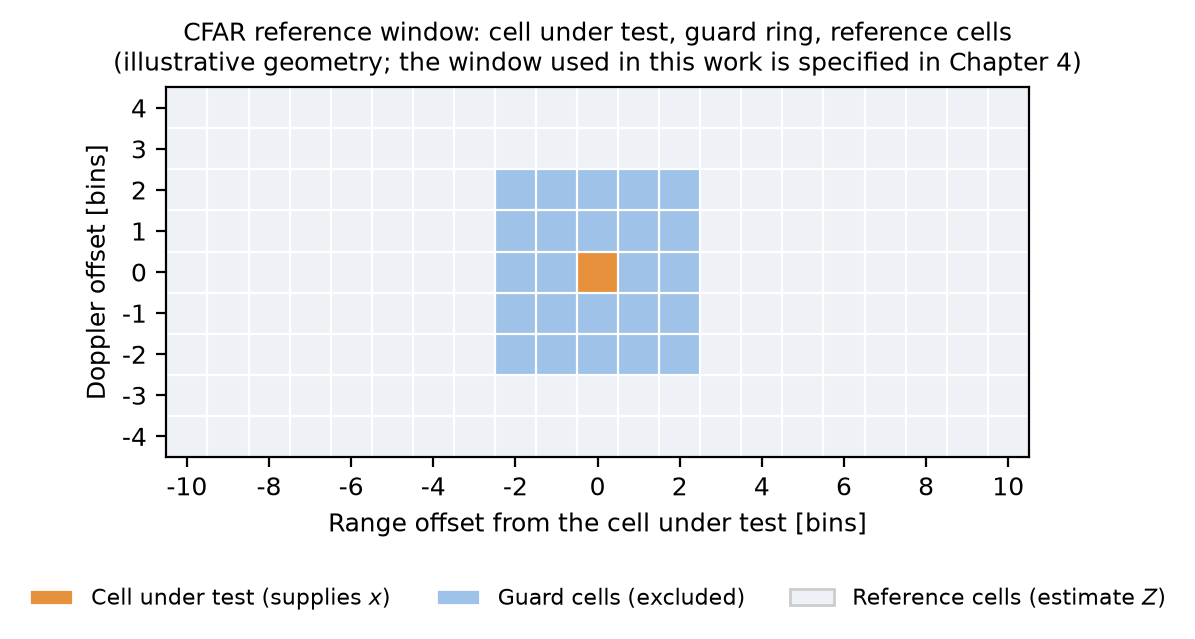
\includegraphics[width=0.95\textwidth]{figures/Chapter2/ch2_fig4_cfar_window.png}
\caption[CFAR reference window geometry]{The three roles a CFAR window assigns to the cells around
each decision. The \textbf{cell under test} supplies the test statistic $x$. The \textbf{guard
cells} immediately surrounding it are excluded, so that a target cannot raise its own threshold.
The remaining \textbf{reference cells} form the background estimate $Z$. The geometry drawn here is
illustrative: the window is rectangular because the two axes of the RD map are not alike, and the
size actually used in this work, together with the reason for it, is specified in
Chapter~\ref{chp:detectors}.}
\label{fig:cfarwin}
\end{figure}

\subsection{Cell-averaging CFAR}

The simplest choice, and the original adaptive-threshold scheme of Finn and
Johnson~\cite{finn1968cfar}, is to average all reference cells,
\begin{equation}
Z_{\mathrm{CA}} = \frac{1}{N} \sum_{i=1}^{N} x_i ,
\end{equation}
where $N$ is the number of reference cells. For square-law detection in homogeneous exponential
noise, the multiplier that achieves a design false-alarm rate is available in closed form:
\begin{equation}
\alpha = N \left( \Pfa^{-1/N} - 1 \right).
\label{eq:alpha_ca}
\end{equation}

Under a specific and quite restrictive set of conditions --- a homogeneous exponential background,
and reference cells that are genuinely free of target energy --- CA-CFAR is optimal in the sense of
maximising $\Pd$ at a given $\Pfa$, because the sample mean is then the most efficient estimator of
the background power~\cite{gandhi1988cfar}. Outside those conditions the optimality claim does not
carry over, and the variants below exist precisely because real backgrounds often violate them.
CA-CFAR is also the cheapest variant, requiring only a sum.

\subsection{Greatest-of, smallest-of and order-statistic variants}

Every CFAR variant differs from CA-CFAR in one respect only: how the reference cells are combined
into $Z$. That single choice determines the variant's strengths and weaknesses.

\begin{description}
\itemsep3pt
\item[GO-CFAR (greatest-of).] The reference cells are split into a leading and a lagging half, and
$Z$ is the larger of the two means~\cite{hansen1980go}. Keeping the higher estimate limits the
increase in false-alarm rate that CA-CFAR shows at a clutter edge, at the cost of masking targets
more readily.
\item[SO-CFAR (smallest-of).] The mirror image: $Z$ is the smaller of the two
half-means~\cite{weiss1982modified}. If an
interfering target contaminates one half, the clean half is used, so closely spaced targets are
resolved. At a clutter edge the estimate is taken from the quieter side, the threshold is set too
low, and the false-alarm rate can increase substantially.
\item[OS-CFAR (order-statistic).] The reference cells are sorted and the $k$-th ranked value is
taken as $Z$, typically with $k \approx 0.75N$~\cite{rohling1983os}. Interfering targets are high outliers and are
excluded by the ranking, which makes the variant robust in multi-target scenes. The cost is a sort
per cell and a small additional loss in homogeneous background.
\end{description}

Analytical threshold relationships exist for GO, SO and OS as well, but they are considerably more
involved than equation~\eqref{eq:alpha_ca}: they depend on the split of the reference cells or on
the distribution of an order statistic, and the published closed forms assume a one-dimensional
window and independent reference cells. Neither assumption holds exactly for the
two-dimensional window and correlated RD background used here. This work therefore obtains all four
multipliers by Monte-Carlo calibration on noise-only data, so that every variant is calibrated
under the same conditions in which it is evaluated. Chapter~\ref{chp:detectors} describes that
procedure and reports the resulting values.

\subsection{Known failure modes}
\label{sec:cfar_failures}

The limitations of these detectors have been understood since Gandhi and
Kassam~\cite{gandhi1988cfar}. Two failure modes dominate, and both follow directly from
equation~\eqref{eq:cfar}: the threshold is only as good as the assumption that the reference cells
describe the background at the cell under test.

\textbf{Clutter edges.} When the window straddles a boundary between two background levels, the
estimate mixes them. On the quiet side of the edge the threshold is set too high and targets are
missed; on the strong side it is set too low and false alarms appear. The threshold cannot follow a
step that is sharper than the window is wide.

\textbf{Target masking.} When a second target falls inside the reference window of the first, it
raises $Z$ and therefore raises the threshold at the very cell being tested. The stronger the
interferer, the more effectively it hides its neighbour.

Figure~\ref{fig:cfarfail} illustrates both mechanisms on a one-dimensional cut, using the same
guard and reference counts per side as the window used in the rest of this work.

\begin{figure}[H]
\centering
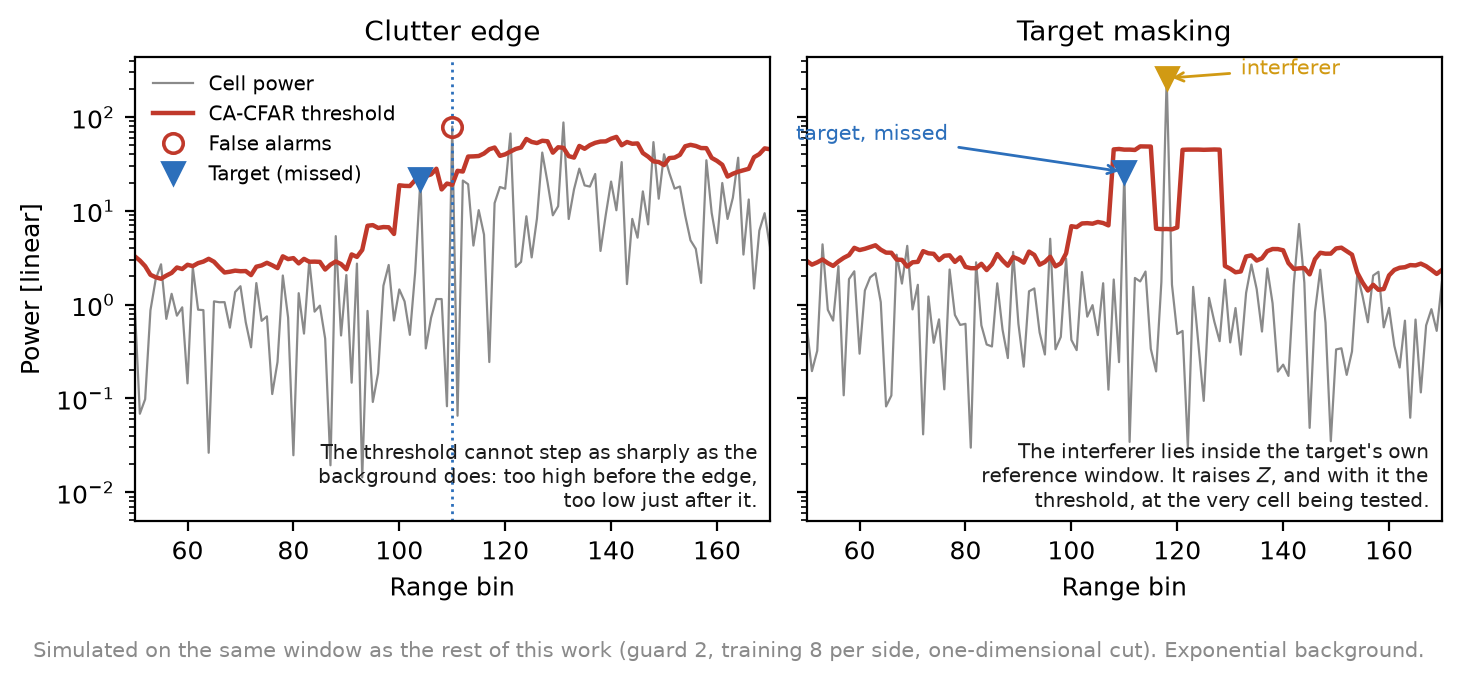
\includegraphics[width=\textwidth]{figures/Chapter2/ch2_fig5_cfar_failure_modes.png}
\caption[The two dominant CFAR failure modes]{\textbf{An illustrative simulation of the two
classical failure mechanisms, not a measured benchmark result.} A one-dimensional cut through an
exponential background is used, with the same guard and reference counts per side as the window of
Figure~\ref{fig:cfarwin}, so that the mechanisms can be seen directly; the outcome for any single
realisation depends on the random draw. Left: at a clutter edge the threshold lags the background
step, missing a target before the edge and admitting a false alarm after it. Right: an interfering
target inside the reference window raises the threshold at the cell being tested, and the weaker
target is missed. Measured performance under these conditions is reported in
Chapter~\ref{chp:synthetic}.}
\label{fig:cfarfail}
\end{figure}

The conclusion Gandhi and Kassam reached is the starting point of this project: no single CFAR
variant performs well across all backgrounds, and each variant tends to repair one failure mode
while worsening another. GO tends to handle clutter edges better than CA but may worsen masking;
SO tends to help in multiple-target cases but can perform poorly at clutter transitions. They
suggested that an adaptive approach might be required when operating conditions change.

These failure modes also determine the design of the benchmark. A comparison evaluated only in
homogeneous noise would test the one condition under which CA-CFAR is already close to optimal, and
would say nothing about the conditions that motivate a learned detector. The conditions used in
Chapter~\ref{chp:synthetic} are chosen to span both.

\subsection{CFAR loss}
\label{sec:cfar_loss}

A third limitation applies even when the background is perfectly homogeneous, so it is not a
failure mode in the sense above.

CFAR estimates the background power from a finite number of reference cells. That estimate is
therefore imperfect, and it varies from one window to the next. To keep the false-alarm rate at its
design value despite this variability, the threshold must be set slightly higher than a detector
that somehow knew the true background power would need. The resulting penalty in signal-to-noise
ratio is called \emph{CFAR loss}~\cite{richards2014radar}. It becomes smaller as the number of
reference cells grows, because the estimate becomes more reliable.

The reason this matters for the present work is that CFAR loss offers a second possible explanation
for any advantage a learned detector shows. The obvious explanation is that the network uses its
local context differently. But a detector that avoids the estimation penalty would also be expected
to do better, even where CFAR has no failure mode at all. Both explanations predict the same
observation, so neither can be accepted without testing the other.
Chapter~\ref{chp:attribution} treats this as one of the candidate mechanisms to be separated
experimentally.

\section{Learned detection on the range--Doppler map}

\subsection{Convolutional detectors}

The RD map is an image-like array, and the detection rule is applied identically at every cell.
Both properties suit a convolutional neural network. A convolutional layer applies the same learned
kernel at every position, which matches the translation invariance of the problem and means the
number of parameters does not grow with the size of the map.

Most learned detectors on RD maps use one of two formulations:

\begin{itemize}
\itemsep2pt
\item \textbf{Patch.} A small window around each cell is extracted and classified on its own. This
mirrors CFAR closely, but it needs one network evaluation per cell.
\item \textbf{Fully convolutional.} The whole map is passed through the network once, producing a
score for every cell in a single pass.
\end{itemize}

The second is far cheaper and is the formulation used in this work. Importantly, processing the
whole map at once does not mean each output depends on the whole map: every output cell still
depends only on the input cells within its receptive field, which is a local neighbourhood set by
the network's depth and kernel sizes.

\subsection{CA-CFAR as a convolution}
\label{sec:cfar_as_conv}

CA-CFAR can be expressed as a fixed convolutional operation followed by
thresholding~\cite{liu2024cacfarconv, banerjee2025rctd}. This provides a useful interpretation for
the comparison in this thesis: both CFAR and TinyCNN map a local neighbourhood to a score, but CFAR
uses a hand-derived fixed rule whereas TinyCNN learns that rule from data. TinyCNN is a richer
nonlinear function rather than a single equivalent CFAR kernel, so the comparison asks whether
learning the local decision rule provides an advantage when spatial context is kept comparable.
Figure~\ref{fig:cfarconv} places the two rules side by side over the same footprint.

\begin{figure}[H]
\centering
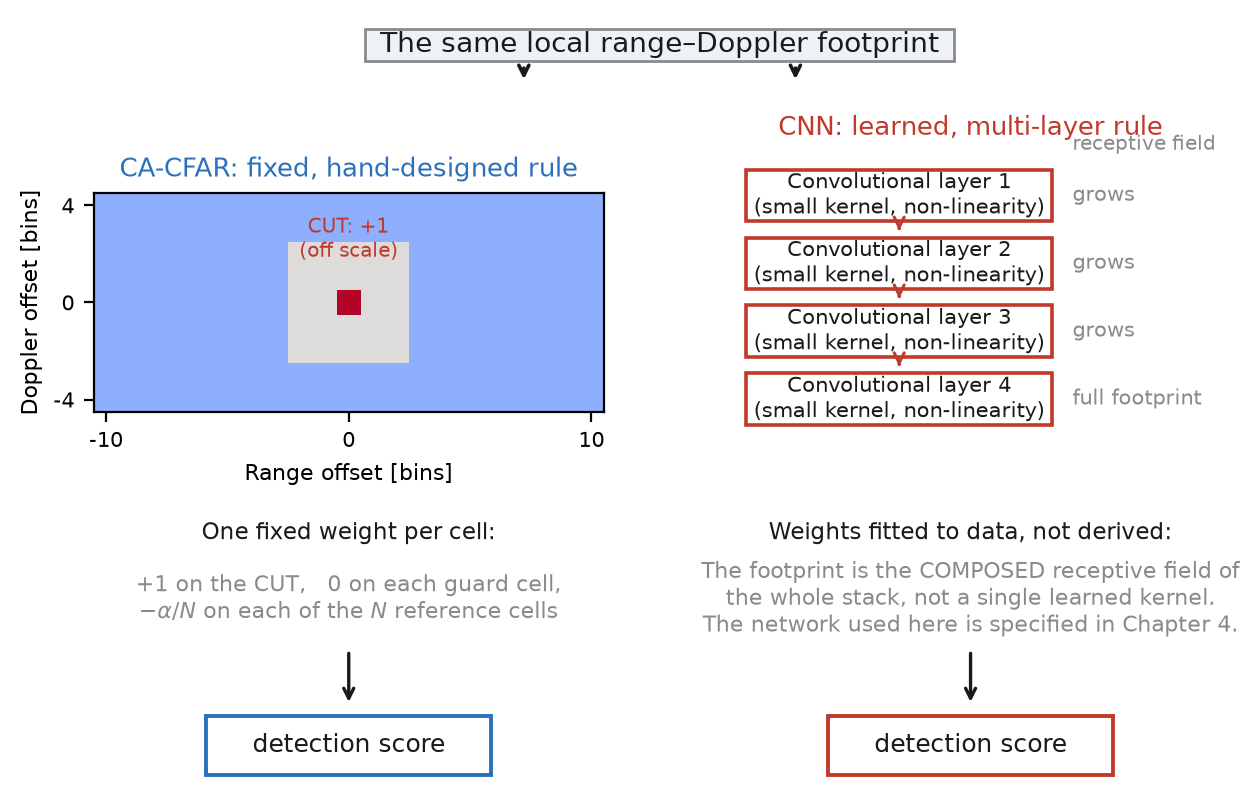
\includegraphics[width=\textwidth]{figures/Chapter2/ch2_fig6_cfar_as_convolution.png}
\caption[A fixed and a learned decision rule over the same footprint]{Both detectors decide from
the same local footprint, but obtain their rule differently. Left: CA-CFAR as one fixed weight per
cell --- $+1$ on the cell under test, $0$ on the guard cells, $-\alpha/N$ on each reference cell
(the colour scale is set by the reference weights, so the cell under test saturates and is labelled
instead). Right: a convolutional network reaches the same footprint by composing several small
convolutions. \textbf{That footprint is the composed receptive field of the whole stack, not a
single learned kernel.}}
\label{fig:cfarconv}
\end{figure}

\subsection{Label representation and supervision}

Unlike CFAR, a learned detector must be given a training target: some representation of where the
targets are. Three forms are common --- a single point, a weighted local region around it, or an
object mask covering the target's support.

The choice is not neutral. It affects both what the network learns to detect and how precisely it
localises, because it defines what a single output cell is being asked to mean. The representation
used in this work, and the reasons for it, are specified in Chapter~\ref{chp:detectors}.

\section{State of the art: learned detectors versus CFAR}
\label{sec:sota}

\subsection{Not every result is directly comparable}

A substantial body of work reports learned detectors outperforming CFAR, and read together the
results appear to show a large and consistent advantage. They do not actually combine, because the
works are solving different tasks: some perform per-cell detection, others object detection with
bounding boxes, others reconstruction or hardware reformulation. A gain reported for one task is
not evidence about another.

Table~\ref{tab:families} groups the reviewed literature accordingly. Only the first family reports
$\Pd$ against CFAR at a matched false-alarm rate on a per-cell decision, which is the quantity this
report measures.

\begin{table}[H]
\centering
\caption{Families in the learned-detection literature. Only the first measures the same quantity as
this work.}
\label{tab:families}
\begin{tabular}{@{}p{3.4cm}p{4.5cm}p{2.6cm}p{2.5cm}@{}}
\toprule
\textbf{Family} & \textbf{Representative work} & \textbf{Metric} & \textbf{Comparable} \\
\midrule
Per-cell learned threshold, scored against CFAR &
RadCNN~\cite{yavuz2021radcnn}, Gusland et al.~\cite{gusland2020deeptemporal},
Lallouet et al.~\cite{lallouet2023loss}, Banerjee et al.~\cite{banerjee2025rctd} &
$\Pd$ at fixed $\Pfa$ &
\textbf{Yes} \\
\addlinespace
CFAR-property constrained learning &
CFARnet~\cite{diskin2023cfarnet} &
ROC, plus a test of the CFAR property &
Partly \\
\addlinespace
Object detection on RD maps &
DAROD~\cite{decourt2022darod} &
mAP at an IoU threshold &
No \\
\addlinespace
Structure-preserving reformulation &
Liu et al.~\cite{liu2024cacfarconv} &
Latency and energy &
No \\
\bottomrule
\end{tabular}
\end{table}

\subsection{The four directly relevant works}

Four studies are particularly relevant to this work, and each for a different reason. RadCNN and
Gusland et al.\ provide direct CNN-versus-CFAR performance comparisons. Lallouet et al.\ motivate
the CFAR-loss hypothesis. Liu et al.\ and Banerjee et al.\ supply the theoretical connection
between fixed CFAR processing and learned convolutional processing.

\subsubsection*{RadCNN: a learned detector does not always win}

RadCNN~\cite{yavuz2021radcnn} evaluates a convolutional detector against CA, GO, SO and OS CFAR on
simulated data with Weibull and K-distributed clutter. Its value here is that the reported outcome
is mixed rather than uniformly favourable. The network gains over CFAR in some clutter conditions.
It ties CFAR in simple homogeneous noise. And it loses in at least one scenario, where the target
lies near clutter but its reference window is filled mostly with noise.

\subsubsection*{Gusland et al.: the closest experimental comparison to this work}

Of the reviewed studies, Gusland et al.~\cite{gusland2020deeptemporal} is the one whose experimental
setup most resembles the present work. They use real X-band FMCW measurements, with a UAV carrying
GPS for ground truth, rather than simulation. They deliberately restrict the network's receptive
field to match the CA-CFAR patch, so that both detectors work from comparable local context.

Their results are consistent with RadCNN. In homogeneous regions the network approximately ties
CFAR. Around clutter transitions it gains roughly $0.25$ to $0.35$ in $\Pd$. That figure is quoted
here because Chapter~\ref{chp:realdata} compares it directly against the clutter-edge result
measured in this work.

\subsubsection*{Lallouet et al.: a proposed explanation for the gains}

Lallouet et al.~\cite{lallouet2023loss} report a learned detector outperforming CFAR on simulated
exoclutter data. Their contribution to this report is not the margin but the explanation they offer
for it: the finite reference window of Section~\ref{sec:cfar_loss} makes CFAR's threshold an
estimate rather than a known quantity, and a learned detector does not pay that penalty.

This is a testable claim, and it is one of the candidate mechanisms examined in the attribution
experiments of Chapter~\ref{chp:attribution}.

\subsubsection*{Liu et al.\ and Banerjee et al.: the structural connection}

These two works are conceptual support rather than a further detector benchmark, and they are cited
for that reason. Liu et al.~\cite{liu2024cacfarconv} show that CA-CFAR can be represented using
convolution-like fixed weights. Banerjee et al.~\cite{banerjee2025rctd} extend the idea towards
learned weights.

Together they support the framing used throughout this report: \textbf{CFAR is a fixed local rule,
and a CNN is a learned local rule}, applied over comparable context.

Two observations run through these comparative studies, and they motivate what follows. Learned
detectors often provide little advantage over a well-configured CFAR in homogeneous conditions but
can gain in more difficult clutter; and the reasons for those gains are not fully established.

\section{Gap addressed by this work}

The review supports four observations, which together define what this project adds. They are
stated briefly here; the underlying fairness arguments were set out in
Section~\ref{sec:problem}.

\begin{enumerate}
\itemsep3pt
\item \textbf{Only a small subset of published work is directly comparable} to the per-cell
CFAR-versus-learned detection task addressed here. Most of the corpus answers a different question.
\item \textbf{Matching the network's spatial context to the CFAR window is uncommon.} Among the
reviewed works only Gusland et al.\ do so deliberately. This work does the same, while stating
explicitly that matching the footprint does not make the two decision rules identical.
\item \textbf{The competing explanations for learned gains are rarely separated experimentally.}
CFAR estimation loss and a different use of local context both predict the same observation, and no
reviewed work distinguishes them. Chapter~\ref{chp:attribution} attempts to.
\item \textbf{Zero-shot synthetic-to-real validation is rarely tested.} Simulation-trained
detectors are almost always evaluated on the same simulator, and measurement-trained detectors on
the same sensor. None of the directly comparable studies identified here evaluates a frozen,
simulation-trained detector on real measurements without retraining. Chapter~\ref{chp:realdata}
reports that evaluation.
\end{enumerate}

\section{Conclusion}

An FMCW radar turns range into a beat frequency and velocity into a phase rotation across chirps,
and two Fourier transforms produce the range--Doppler map on which detection is performed. CFAR
detects by estimating the local background from a reference window and applying an adaptive
threshold proportional to it; its variants --- CA, GO, SO and OS --- differ only in how that
estimate is formed, and each has different strengths and weaknesses across homogeneous background,
clutter edges and multiple targets.

One idea from this chapter carries into the rest of the report: \textbf{CFAR is a fixed local
operator applied to a neighbourhood of each cell, and a convolutional network is a learned local
operator over comparable context}. That framing is what makes the comparison in this report a
controlled one. Two questions are left open by the reviewed work --- why the reported learned gains
occur, and whether they survive a change of domain --- and they motivate the experiments that follow.
Chapter~\ref{chp:simulator} begins by specifying the simulator and the datasets, chosen so that the
conditions identified in Section~\ref{sec:cfar_failures} are represented and so that the
range--Doppler geometry matches the real dataset used later.
